\documentclass[12pt]{article}

\usepackage{mathtools}
\usepackage{listings}
\usepackage{enumerate}
\usepackage{xcolor}
\usepackage{xspace}
\usepackage{graphicx}
\usepackage{subcaption}
\usepackage{adjustbox}
\usepackage{booktabs}
\usepackage[italian]{babel}
\usepackage[utf8]{inputenc}
\usepackage[T1]{fontenc}
\usepackage{float}
\usepackage{caption}
\usepackage[shortlabels]{enumitem}

\usepackage{mathpazo} 
\definecolor{codeblue}{rgb}{0.21, 0.46, 0.80}
\definecolor{backcolour}{rgb}{0.96,0.96,0.93}
\definecolor{monokai@black}{HTML}{2C2C2A}
\definecolor{monokai@gray}{HTML}{524F52}
\definecolor{monokai@magenta}{HTML}{D33682}
\definecolor{monokai@blue}{HTML}{004C99}


\lstdefinestyle{matlab}{
	frame=tb,
	language=Matlab,
	backgroundcolor=\color{backcolour},
	aboveskip=3mm,
	belowskip=3mm,
	showstringspaces=false,
	columns=flexible,
	basicstyle={\small\ttfamily},
	numbers=left,
	numberstyle=\tiny\color{monokai@black},
	numbersep=7pt,
	stepnumber=2,
	breaklines=true,
	breakatwhitespace=true,
	tabsize=3,
	numberstyle=\color{monokai@gray},
	keywordstyle=\color{codeblue},
	stringstyle=\color{monokai@magenta}\ttfamily,
	identifierstyle=\color{monokai@black},
	commentstyle=\color{monokai@blue},
	emphstyle=\color{monokai@red},
	columns=fullflexible,
	morekeywords={symfun, syms}
}

\renewcommand{\lstlistingname}{Codice}
\newcommand{\MATLAB}{\textsc{Matlab }}

\newcommand{\myItalianTitle}{Interpolazione di superfici alla Hermite}
\newcommand{\myDegree}{Corso di Laurea in Informatica\xspace}

\newcommand{\myName}{Filippo Mameli\xspace}
\newcommand{\myFaculty}{Scuola di Scienze Matematiche, Fisiche e Naturali\xspace}
\newcommand{\myUni}{\protect{Universit\`a degli Studi di Firenze}\xspace}
\newcommand{\myLocation}{Firenze\xspace}
\newcommand{\myTime}{Anno Accademico 2018-2019\xspace}
\newcommand{\myVersion}{Version 0.1\xspace}

\begin{document}
\begin{titlepage}
	\begin{center}
   	\large
      \hfill
      \vfill
      \begingroup
         \includegraphics[scale=0.3]{img/LOGO.pdf}\\
%			\spacedallcaps{\myUni} \\
			\myFaculty \\
			\myDegree \\
			\vspace{0.5cm}
      \endgroup
      \vfill
      \begingroup
		  \myItalianTitle \\ 
	\bigskip
      \endgroup
      \myName
      \vfill
      \vfill
      Relatore: \emph{Rosario Pugliese}\\
      Correlatore: \emph{Andrea Margheri}\\
      \vfill
      \vfill
      \myTime
      \vfill
	\end{center}
\end{titlepage}
%--------------------------------------------------------------
% back titlepage
%--------------------------------------------------------------
   \newpage
	\thispagestyle{empty}
	\hfill
	\vfill
	\noindent\myName:
	\textit{\myItalianTitle,}
	\myDegree, \textcopyright\ \myTime


\section{Patch bicubico interpolante alla Hermite}

L'interpolazione di Hermite a differenza dell'interpolazione di Lagrande si basa non solo
sull'utilizzo dei punti della funzione vettoriale, ma aggiunge anche come parametri in input
anche le derivate parziali e miste. Il patch bicubico nella forma di Hermite è dato da:

$$ X(u,v) = \sum_{i=0}^{3}\sum_{j=0}^{3} h_{ij}H_3^3(u)H_3^3(v); \hspace{1em} 0 \geq u, v \geq 1;$$
dove $H_i^3$ sono le funzioni cubiche di Hermite definite nel modo seguente:
$$H^3_0(t) = 1 - 3t^2 + 2t^3; H^3_1(t) = t -2t^2 + t^3; H^3_2(t) = t^3 - t^2; H^3_3(t) = 3t^2 - 2t^3.$$
I valori di $h_{ij}$ sono dati dalla matrice:

$$\mathbf{C} = 
\begin{pmatrix}
    \mathbf{X}(0,0)     & \mathbf{X}_t(0,0)     & \mathbf{X}_t(0,1)     & \mathbf{X}(0,1) \\
    \mathbf{X}_s(0,0)   & \mathbf{X}_{st}(0,0)  & \mathbf{X}_{st}(0,1)  & \mathbf{X}_s(0,1) \\
    \mathbf{X}_s(1,0)   & \mathbf{X}_{st}(1,0)  & \mathbf{X}_{st}(1,1)  & \mathbf{X}_s(1,1) \\
    \mathbf{X}(1,0)     & \mathbf{X}_t(1,0)     & \mathbf{X}_t(1,1)     & \mathbf{X}(1,1) 
\end{pmatrix}  $$
La matrice può essere vista come 4 gruppi di matrici 2x2 contenenti le informazioni
sui angoli del patch.

\begin{figure}[H]
    \centering

    \includegraphics[scale=0.7]{img/der.png}

    \caption{Rappresentazione dei punti e dei vettori}\label{fig:1}
\end{figure}

\section{Implementazione in Matlab}
Per testare il codice scegliamo come superficie il toroide in Figura~\ref{fig:1}.
Da questo prendiamo una porzione più piccola per ricavare i dati da usare in input
per l'interpolazione.

\begin{figure}[H]
    \centering

    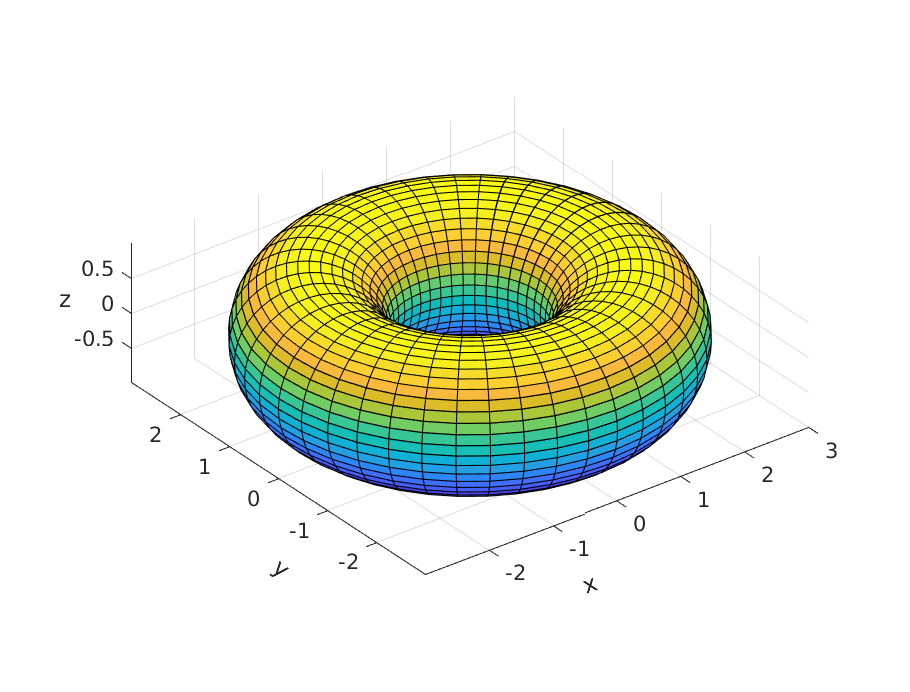
\includegraphics[scale=0.7]{img/toro.eps}

    \caption{Rappresentazione dei punti e dei vettori}\label{fig:2}
\end{figure}

La superficie del toro è stata disegnata eseguendo il Codice~\ref{toro}
\begin{lstlisting}[caption={Plot del toro}, style=matlab, label={toro}, captionpos=b]
s_a = 0; s_b = 7;
s = linspace(s_a, s_b, 50);
t_a = 0; t_b = 7;
t = linspace(t_a, t_b, 50);
[ss, tt] = meshgrid(s, t);
x = (2 + cos(tt)).*cos(ss);
y = (2 + cos(tt)).*sin(ss);
z = sin(tt);
surf(x, y, z);axis equal; xlabel('x', 'Rotation',20); ylabel('y', 'Rotation',-20); zlabel('z', 'Rotation',0);
\end{lstlisting}
Prendiamo solo una porzione della superficie delimitata dai parametri $s_a$, $s_b$, $t_a$ e $t_b$.
Su questa con il Codice~\ref{angoli} visualiziamo in Figura~\ref{fig:3} i quattro angoli che useremo per la costruzione
della matrice di Hermite.

\begin{figure}[H]
    \centering

    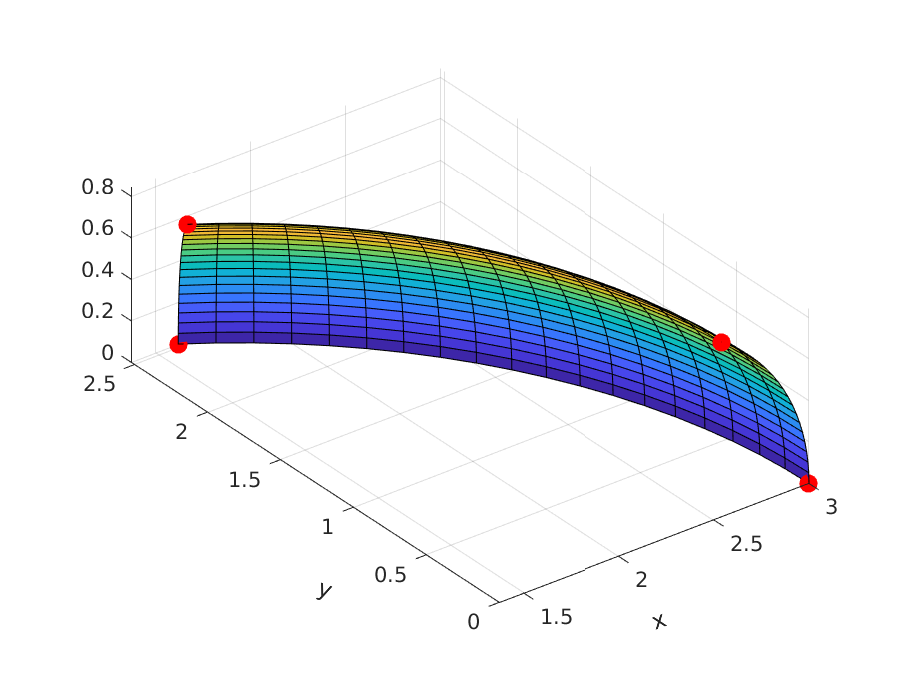
\includegraphics[scale=0.7]{img/cornerPatch.eps}

    \caption{Angoli della porzione di toro}\label{fig:3}
\end{figure}

\begin{lstlisting}[caption={Visualizzazione dei 4 angoli della porzione di toro}, style=matlab, label={angoli}, captionpos=b]
cx_1 = (2 + cos(t_a)).*cos(s_a);
cy_1 = (2 + cos(t_a)).*sin(s_a);
cz_1 = sin(t_a);

cx_2 = (2 + cos(t_b)).*cos(s_a);
cy_2 = (2 + cos(t_b)).*sin(s_a);
cz_2 = sin(t_b);

cx_3 = (2 + cos(t_b)).*cos(s_b);
cy_3 = (2 + cos(t_b)).*sin(s_b);
cz_3 = sin(t_b);

cx_4 = (2 + cos(t_a)).*cos(s_b);
cy_4 = (2 + cos(t_a)).*sin(s_b);
cz_4 = sin(t_a);

surf(x, y, z);axis equal; xlabel('x', 'Rotation',20); ylabel('y', 'Rotation',-20); hold on;
plot3(cx_1, cy_1, cz_1, 'r.', 'MarkerSize', 30);
plot3(cx_2, cy_2, cz_2, 'r.', 'MarkerSize', 30);
plot3(cx_3, cy_3, cz_3, 'r.', 'MarkerSize', 30);
plot3(cx_4, cy_4, cz_4, 'r.', 'MarkerSize', 30);
\end{lstlisting}
La matrice $\mathbf{C}$ è una matrice a tre piani ciascuno 4x4. Per ricavare i valori delle 
derivate parziali e miste utilizziamo il \textit{Symbolic Math Toolbox} di \MATLAB.
Definiamo le funzioni $f(x)$, $f(y)$ e $f(z)$ e i parametri $s$ e $t$. Nel Codice~\ref{derivate}
si può vedere come utilizzando la funzione \textit{diff} si possa ricavare le derivate sui
parametri $s$, $t$ oppure $s$ e $t$ per ognuna delle funzioni definite.
\begin{lstlisting}[caption={Derivate delle funzioni della superficie}, style=matlab, label={derivate}, captionpos=b]
C = zeros(4,4,3);
syms s t f_x(s,t) f_y(s,t) f_z(s,t)

f_x(s,t) = (2 + cos(t)).*cos(s);
f_y(s,t) = (2 + cos(t)).*sin(s);
f_z(s,t) = sin(t);

df_xt = diff(f_x, t);
df_xs = diff(f_x, s);
df_xst = diff(f_x, s, t);

df_yt = diff(f_y, t);
df_ys = diff(f_y, s);
df_yst = diff(f_y, s, t);

df_zt = diff(f_z, t);
df_zs = diff(f_z, s);
df_zst = diff(f_z, s, t);	
\end{lstlisting}
Per ogni piano della matrice la costruzione è uguale. Nel Codice~\ref{matriceCX} vediamo in dettaglio la definizione del piano $X$. 
\newpage \noindent
Analizzando i 4 elementi nell'angolo in alto a sinistra della matrice vediamo che:
\begin{itemize}[-]
	\item Nella posizione (1, 1) abbiamo il punto di interpolante;
	\item Nelle posizioni (1, 2) e (2, 1) abbiamo i valori delle funzioni derivate rispettivamente per $t$ e per $s$ in $s_a$ e $t_a$;
	\item Nella posizione (2, 2) abbiamo il valore della funzione derivata mista in $s_a$ e $t_a$;
\end{itemize}

\begin{lstlisting}[caption={Definizione del piano $X$ della matrice C}, style=matlab, label={matriceCX}, captionpos=b]
C_x = zeros(4,4);
C_x(1,1) = f_x(s_a, t_a);
C_x(1,2) = df_xt(s_a, t_a);
C_x(2,1) = df_xs(s_a, t_a);
C_x(2,2) = df_xst(s_a, t_a);

C_x(1,4) = f_x(s_a, t_b);
C_x(1,3) = df_xt(s_a, t_b);
C_x(2,4) = df_xs(s_a, t_b);
C_x(2,3) = df_xst(s_a, t_b);

C_x(4,1) = f_x(s_b, t_a);
C_x(4,2) = df_xt(s_b, t_a);
C_x(3,1) = df_xs(s_b, t_a);
C_x(3,2) = df_xst(s_b, t_a);

C_x(4,4) = f_x(s_b, t_b);
C_x(4,3) = df_xt(s_b, t_b);
C_x(3,4) = df_xs(s_b, t_b);
C_x(3,3) = df_xst(s_b, t_b);
\end{lstlisting}
Iterando lo stesso procedimento per i piani $Y$ e $Z$ della matrice $\mathbf{C}$ possiamo passare al calcolo della patch
in forma di Hermite.
Utilizzando il calcolo matriciale abbiamo:

$$\mathbf{X}(s,t) = \mathbf{H}^T(s)\mathbf{\ C\ H}(t)$$\\
dove $\mathbf{H}(t) = (H^3_0(t), H^3_1(t), H^3_2(t), H^3_3(t))$.\\
Nel Codice~\ref{patchHermite} vediamo prima la definizione delle funzioni della base di
Hermite per poi passare calcolo di $X(s,t)$. In Figura~\ref{fig:4} viene mostrata la porzione
di superficie disegnata utilizzando il patch bicubico ricavato.
\begin{lstlisting}[caption={Patch in forma di Hermite}, style=matlab, label={patchHermite}, captionpos=b]
syms H_0_t(t) H_1_t(t) H_2_t(t) H_3_t(t) H_0_s(s) H_1_s(s) H_2_s(s) H_3_s(s)

H_0_t(t) = 1 - 3*t.^2 + 2.*t.^3;
H_1_t(t) = t - 2*t.^2 + t.^3;
H_2_t(t) = t.^3 - t.^2;
H_3_t(t) = 3*t.^2 - 2*t.^3;

H_0_s(s) = 1 - 3*s.^2 + 2*s.^3;
H_1_s(s) = s - 2*s.^2 + s.^3;
H_2_s(s) = s.^3 - s.^2;
H_3_s(s) = 3*s.^2 - 2*s.^3;

H_t = [H_0_t(t); H_1_t(t); H_2_t(t); H_3_t(t)];
H_s = [H_0_s(s); H_1_s(s); H_2_s(s); H_3_s(s)];

X_st = symfun((H_s.') * C(:,:,1) * H_t, [s,t]);
Y_st = symfun((H_s.') * C(:,:,2) * H_t, [s,t]);
Z_st = symfun((H_s.') * C(:,:,3) * H_t, [s,t]);
\end{lstlisting}

\begin{figure}[H]
    \centering

    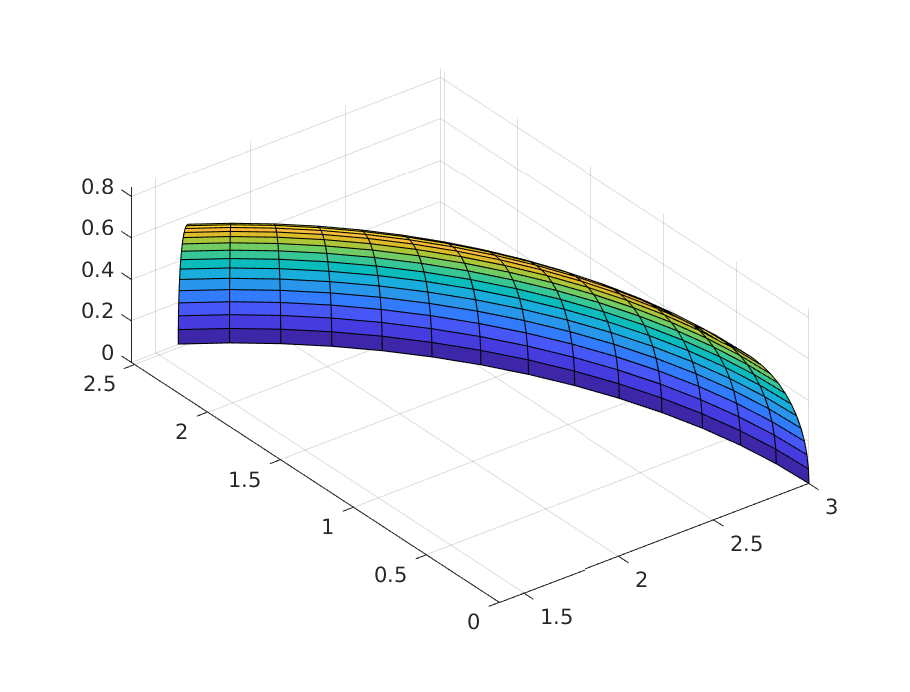
\includegraphics[scale=0.7]{img/hermitePatch.eps}

    \caption{Patch in forma di Hermite}\label{fig:4}
\end{figure}


\section{Errore di interpolazione}
\label{sec:errori}
In questo sezione analiziamo l'errore di interpolazione confrontando i valori esatti della superficie con i valori del patch interpolante. 
I parametri $s_a$, $s_b$, $t_a$ e $t_b$ presi per eseguire
i test appartengono a $[0,1]^2$, utilizzando questi valori la norma 2 calcolata con il Codice~\ref{error}
risulta:
\begin{itemize}[-]
	\item per x: 0.0717;
	\item per y: 0.0396;
	\item per z: 0.0114
\end{itemize}
data l'ampiezza del dominio parametrico-$st$ i valori degli errori sono quelli che ci potevamo aspettare,
passando da $[0,1]^2$ a $[0,0.5]^2$ abbiamo invece dei valori di norma 2 pari a:
\begin{itemize}[-]
	\item per x: 0.0016;
	\item per y: 4.1487e-04;
	\item per z: 1.1477e-04.
\end{itemize}
L'errore in questo caso diminuisce notevolmente.
Questo ci fa capire che questa tecnica di interpolazione è molto più efficace prendendo domini
parametrici piccoli. Nella Sessione~\ref{sec:erroriSpline} vedremo come la divisione in sottointervalli 
sempre più piccoli porterà alla diminuzione e all'annullamento dell'errore.
\begin{lstlisting}[caption={Norma 2}, style=matlab, label={error}, captionpos=b]
norm(abs(X_hermite - X))
norm(abs(Y_hermite - Y))
norm(abs(Z_hermite - Z))
\end{lstlisting}

\section{Dalla forma di Hermite alla forma di Bezier}
Possiamo passare con dei semplici calcoli dalla forma di Hermite alla forma di Bezier
in modo tale da utilizzare l'algoritmo di de Casteljau per la tabulazione.
Il patch in forma di Bezier è così definito:

$$\mathbf{X}(s,t) = \mathbf{B}^T(s)\mathbf{\ M \ B}(t)$$
con\\
$$B^3_0(t) = (1 - t)^3, B^3_1(t) = 3t(1 - t)^2 B^3_2(t) = 3t^2(1 - t), B^3_3(t) = t^3$$
\noindent
dove
$$\mathbf{B}(t) = (B^3_0(t), B^3_1(t), B^3_2(t), B^3_3(t))$$
e $\mathbf{M}$ è una matrice a 4x4 a tre piani.

Data la matrice di Hermite possiamo ad ogni elemento associare una posizione della matrice 
nella forma di Bezier.
Utilizziamo il Codice~\ref{bezier_matrix} per ricavare da un piano della matrice di Hermite
il piano della matrice associato per forma di Bezier.
\lstinputlisting[caption={Matrice di Bezier}, style=matlab, label={bezier_matrix}, captionpos=b]{../bezier_matrix.m}
Riprodotto questo procedimento per tutti e tre i piani, come mostrato nel Codice~\ref{full_bezier}, possiamo
passare alla definizione del patch in forma di Bezier.
\lstinputlisting[caption={Matrice di Bezier completa}, style=matlab, label={full_bezier}, captionpos=b]{../full_bezier_matrix.m}
Nello stesso modo del patch di Hermite definiamo le funzioni di base per scrivere
in forma matriciale il patch di Bezier. 
Visualiziamo nel Codice~\ref{patchBezier} come sono state create le funzioni del patch.
\begin{lstlisting}[caption={Patch in forma di Bezier}, style=matlab, label={patchBezier}, captionpos=b]
syms  Ber_0_t(t) Ber_1_t(t) Ber_2_t(t) Ber_3_t(t) Ber_0_s(s) Ber_1_s(s) Ber_2_s(s) Ber_3_s(s)
Ber_0_t(t) = (1 - t).^3;
Ber_1_t(t) = 3*t*(1 - t).^2;
Ber_2_t(t) = 3*t.^2*(1 - t);
Ber_3_t(t) = t.^3;

Ber_0_s(s) = (1 - s).^3;
Ber_1_s(s) = 3*s*(1 - s).^2;
Ber_2_s(s) = 3*s.^2*(1 - s);
Ber_3_s(s) = s.^3;

Ber_t = [Ber_0_t(t); Ber_1_t(t); Ber_2_t(t); Ber_3_t(t)];
Ber_s = [Ber_0_s(s); Ber_1_s(s); Ber_2_s(s); Ber_3_s(s)];

XB_st = symfun((Ber_s.') * M(:,:,1) * Ber_t, [s,t]);
YB_st = symfun((Ber_s.') * M(:,:,2) * Ber_t, [s,t]);
ZB_st = symfun((Ber_s.') * M(:,:,3) * Ber_t, [s,t]);
\end{lstlisting}
Su questo nuovo patch possiamo fare un controllo di equivalenza con il patch in forma di Hermite.
Nel Codice~\ref{controlloEqui} vediamo come a meno di una tolleranza e assumendo che lo spazio
parametrico sia compreso tra i valori presi in considerazione, i due patch bicubici sono uguali.
\begin{lstlisting}[caption={Controllo di equivalenza tra i due patch}, style=matlab, label={controlloEqui}, captionpos=b]
assume(s_a <= s <= s_b)
assume(t_a <= t <= t_b)
isAlways(abs(X_st - XB_st) <  1.0e-13 )
isAlways(abs(Y_st - YB_st) <  1.0e-13 )
isAlways(abs(Z_st - ZB_st) <  1.0e-13 )
\end{lstlisting}
Scriviamo l'algoritmo di de Casteljau in modo da sfruttare la forma di Bezier del patch. 
Utilizzando l'algoritmo i tempi per la tabulazione si riducono notevolmente. 
Passiamo dai 5 secondi della forma matriciale con il calcolo simbolico, a meno di un secondo
utilizzando de Casteljau. In Figura~\ref{fig:5} viene visualizzata la superficie calcolata
e i nodi del patch. L'algoritmo di de Casteljau bivariato sul patch viene eseguito tramite il 
Codice~\ref{deCasteljau2} che richiama il Codice~\ref{deCasteljau} di de Casteljau monovariato.
\begin{figure}[H]
    \centering

    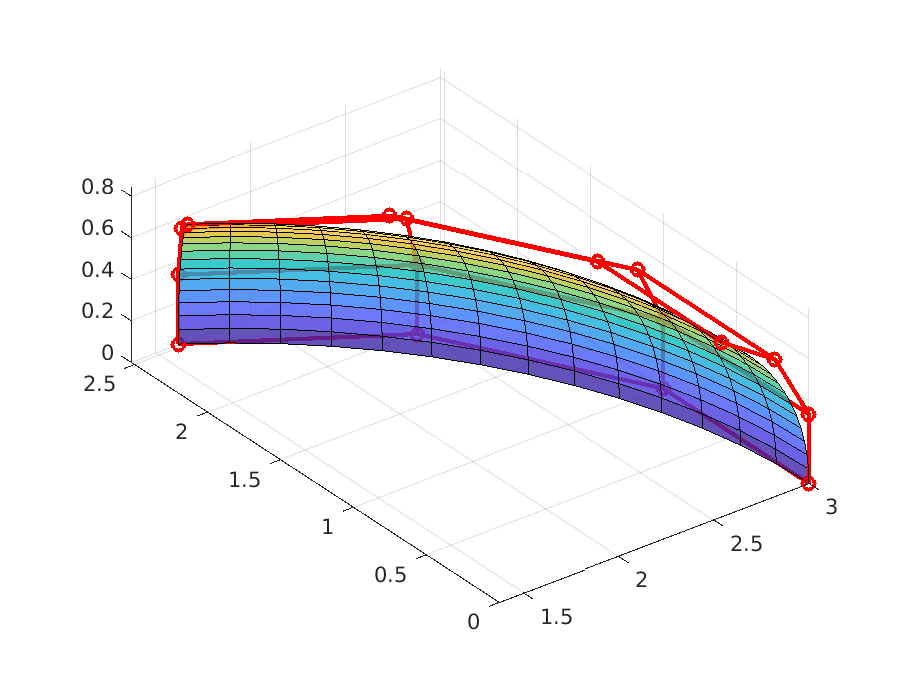
\includegraphics[scale=0.7]{img/deCasteljauPatch.eps}

    \caption{Plot dei nodi e della superficie calcolata con de Casteljau}\label{fig:5}
\end{figure}

\lstinputlisting[caption={Algoritmo di de Casteljau per la superficie}, style=matlab, label={deCasteljau2}, captionpos=b]{../deCasteljau2.m}
\lstinputlisting[caption={Algoritmo di de Casteljau a un solo parametro}, style=matlab, label={deCasteljau}, captionpos=b]{../deCasteljau.m}

\section{Generalizzazion al caso spline}
Utilizziamo l'unione di tanti patch per definire la superficie.
Ogni patch è definito un un sottorettangolo del dominio parametrico.
Determiniamo la superficie $\mathbf{X} \ : \ A \rightarrow E^3$ tale che,
$\forall i = 0, \dots , n$ e $\forall j = 0, \dots , m$ risulti
$$\mathbf{X}(u_i, v_j) = \mathbf{P}_{i,j}, \ \mathbf{X}_u(u_i, v_j) = \mathbf{d}_{i,j}^{(1,0)} \  \mathbf{X}_v(u_i, v_j) = \mathbf{d}_{i,j}^{(0,1)} \  \mathbf{X}_{uv}(u_i, v_j) = \mathbf{d}_{i,j}^{(1,1)}.$$
Poniamo inoltre la divisione in patch,
$$\mathbf{X}(u, v) = \mathbf{X}^{(i,j)}(u, v),\  \text{se}\  u \in [u_i, u_{i+1}],\ \text{e} \ v \in [v_j, v_{j+1}].$$
Posto
$$ s = \frac{u-u_i}{\Delta u_i}, t = \frac{v - v_j}{\Delta v_j} \hspace{2em} (\text{parametri locali})$$
con $\Delta u_i = u_{i+1} - u_i$ e $\Delta u_i = u_{i+1} - u_i$, utilizzando queste due variabili
possiamo scrivere $\mathbf{X^{(i,j)}}(s,t = \mathbf{H}^T(s)\ \mathbf{C}(i,j)) \ \mathbf{H}(t).$
Per imporre le 4 x 4 condizioni di interpolazione sugli estremi del sotto-rettangolo in cui risulta definita $\mathbf{X}^{(i,j)}$, si pone allora

$$\mathbf{C}^{(i,j)} = 
\begin{pmatrix}
\mathbf{P}_{i,j}                     & \Delta v_j\mathbf{d}_{i,j}^{(0,1)}             & \Delta v_j\mathbf{d}_{i,j+1}^{(0,1)}             & \mathbf{P}_{i,j+1} \\
\Delta u_i\mathbf{d}_{i,j}^{(1,0)}   & \Delta u_i\Delta v_j\mathbf{d}_{i,j}^{(1,1)}   & \Delta u_i\Delta v_j\mathbf{d}_{i,j+1}^{(1,1)}   & \Delta u_i\mathbf{d}_{i,j+1}^{(0,1)} \\
\Delta u_i\mathbf{d}_{i+1,j}^{(1,0)} & \Delta u_i\Delta v_j\mathbf{d}_{i+1,j}^{(1,1)} & \Delta u_i\Delta v_j\mathbf{d}_{i+1,j+1}^{(1,1)} & \Delta u_i\mathbf{d}_{i+1,j+1}^{(0,1)} \\
\mathbf{P}_{i+1,j}                   & \Delta v_j\mathbf{d}_{i+1,j}^{(0,1)}           & \Delta v_j\mathbf{d}_{i+1,j+1}^{(0,1)}           & \mathbf{P}_{i+1,j+1} 
\end{pmatrix}  $$
Nel Codice~\ref{matrixSpline} viene descritta la funzione \MATLAB per definire la matrice della forma di Hermite
nel caso spline.
\lstinputlisting[caption={Matrice della forma di Hermite caso spline}, style=matlab, label={matrixSpline}, captionpos=b]{../hermite_matrix_spine.m}

Dividiamo il dominio parametrico di $u$ in tre parti, $[0 \ 0.5 \ 0.9 \ 1]$. 
Nella Figura~\ref{fig:6} vediamo come l'unione dei patch formi la superficie di partenza.
Notiamo che il patch (in blu) definito nel dominio $u_1 = [0 \ 0.5]$ è quello più grossolano
mentre il patch (in giallo) definito nel dominio $u_3 = [0.9 \ 1]$ è quello più fitto.

\begin{figure}[H]
    \centering

    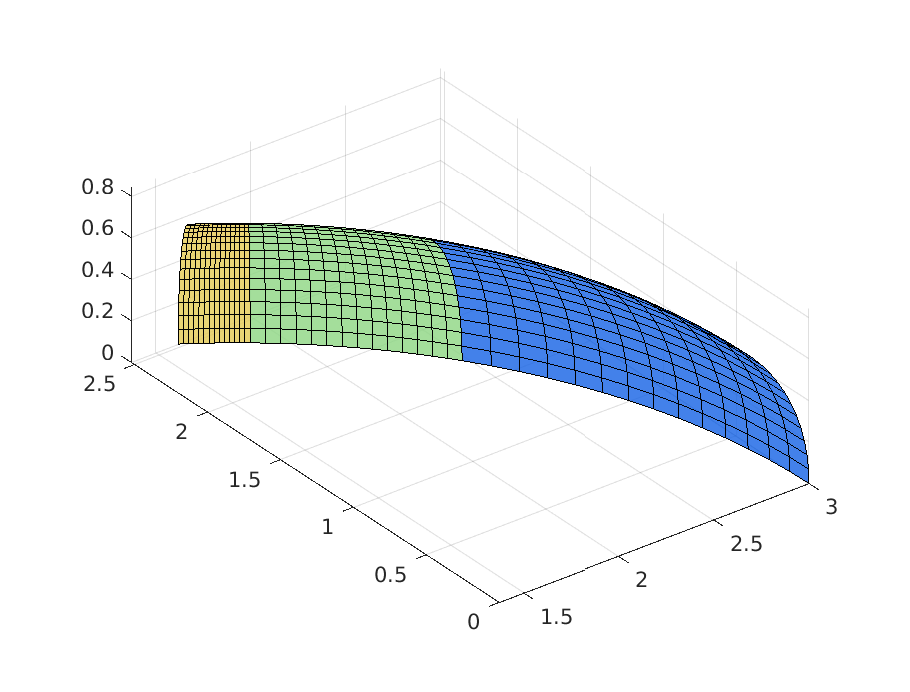
\includegraphics[scale=0.7]{img/splinePatch.eps}

    \caption{Patch spline}\label{fig:6}
\end{figure}

Usando tutto il dominio parametrico della superficie e dividendolo in 16 parti, vediamo in
Figura~\ref{fig:7} tutta la superficie definita dall'unione di 16 patch in forma di Hermite.
\begin{figure}[H]
    \centering

    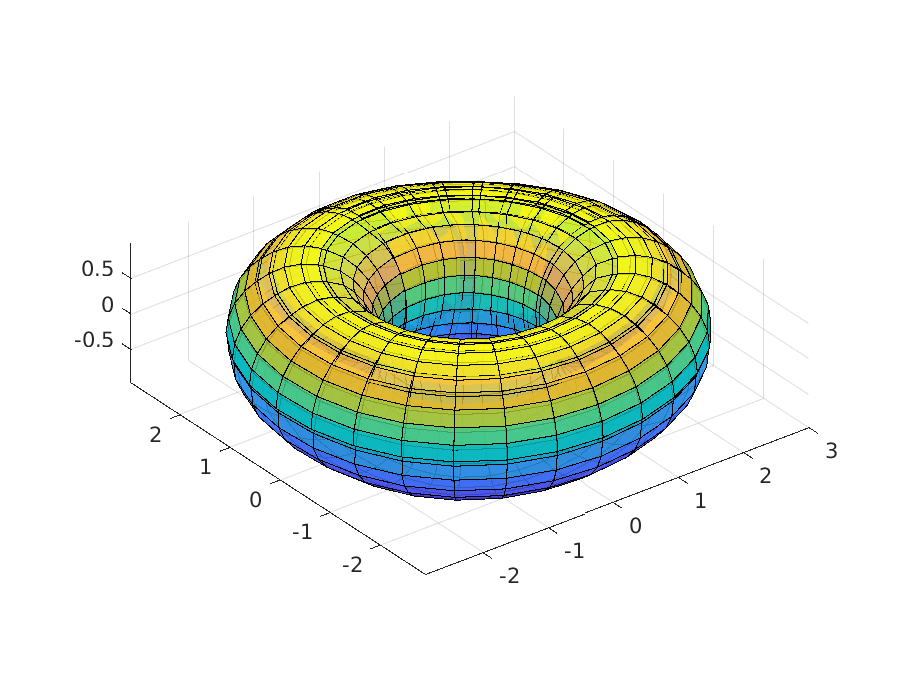
\includegraphics[scale=0.7]{img/splineFullPatch.eps}

    \caption{Superficie intera }\label{fig:7}
\end{figure}

\section{Errore di interpolazione caso spline}\label{sec:erroriSpline}
Prendendo il patch nel dominio parametrico $[0, 1]^2$ nel caso base ($n = 1$ e $m = 1$)
abbiamo ovviamente gli stessi valori di errore:
\begin{itemize}[-]
	\item per x: 0.0717;
	\item per y: 0.0396;
	\item per z: 0.0114;
\end{itemize}
Dividendo il dominio in due parti il dominio su $u$ ($n = 2$ e $m = 1$) abbiamo i seguenti valori:
\begin{itemize}[-]
	\item per x: 0.0201;
	\item per y: 0.0114;
	\item per z: 0.0114;
\end{itemize}
Dividendo il dominio anche su $v$ ($n = 2$ e $m = 2$) abbiamo:
\begin{itemize}[-]
	\item per x: 0.0113;
	\item per y: 0.0136;
	\item per z: 6.9577e-04;
\end{itemize}

Dividendo ulteriormente il dominio sia su $u$ che su $v$ ($n = 3$ e $m = 3$) abbiamo:
\begin{itemize}[-]
	\item per x: 0.0054;
	\item per y: 0.0075;
	\item per z: 1.3694e-04;
\end{itemize}
Nell'ultimo caso abbiamo diviso la superficie in 9 sottopatch. 
Nel Codice~\ref{patchnm9} troviamo lo script \MATLAB per il calcolo nell'errore

\begin{figure}[H]
    \centering

    \includegraphics[scale=0.5]{img/spline3nmpatch.png}

    \caption{Superficie unione di 9 patch }\label{fig:8}
\end{figure}
\newpage
\begin{lstlisting}[caption={Errore interpolazione caso spline}, style=matlab, label={patchnm9}, captionpos=b]
	n = 3; m = 3;
	indexes_i = linspace(1, n, n);
	indexes_j = linspace(1, m, m);
	prec = 15;
	u_i = linspace(0, 1, n + 1);v_j = linspace(0, 1, m + 1);
	du_i = zeros(1, n);dv_j = zeros(1, m);
	for k = indexes_i
		du_i(k) = u_i(k + 1) - u_i(k);
	end
	for k = indexes_j
		dv_j(k) = v_j(k + 1) - v_j(k);
	end
	X_norms = [];Y_norms = [];Z_norms = [];
	colors = [[107, 98, 229];[141, 214, 130];[227, 201, 83]]/255;	
	for i = indexes_i
		for j = indexes_j
			C = full_hermite_matrix_spine(f_x, f_y, f_z, u_i(i), u_i(i + 1), v_j(j), v_j(j + 1), du_i(i), dv_j(j));
			P = full_bezier_matrix(C(:,:,1),C(:,:,2),C(:,:,3));
			[X_hermite, Y_hermite, Z_hermite] = plotDeCasteljau(P, prec);
			surf(X_hermite, Y_hermite, Z_hermite, 'FaceAlpha', .8, 'FaceColor', colors(mod(i,3)+1,:)); axis equal;hold on;
			u = linspace(u_i(i), u_i(i + 1), prec);
			v = linspace(v_j(j), v_j(j + 1), prec);
			[uu, vv] = meshgrid(u, v);
			X = (2 + cos(vv)).*cos(uu);
			Y = (2 + cos(vv)).*sin(uu);
			Z = sin(vv);
			X_norms(end + 1) = norm(abs(X_hermite - X'));
			Y_norms(end + 1) = norm(abs(Y_hermite - Y'));
			Z_norms(end + 1) = norm(abs(Z_hermite - Z'));
		end
	end
	mean(X_norms)
	mean(Y_norms)
	mean(Z_norms)
\end{lstlisting}
\end{document}\documentclass[12pt]{article}